% ============================================================
%  SENTINEL-GNSS — Individual Report: Ogunlade Joshua (LS2525237)
%  Beihang University H3I  ·  Team Pilot Project  ·  2025
%
%  Compile: pdflatex -> bibtex -> pdflatex -> pdflatex
% ============================================================
\documentclass[12pt,a4paper]{article}

\usepackage[T1]{fontenc}
\usepackage[utf8]{inputenc}
\usepackage{lmodern}
\usepackage{microtype}
\usepackage[top=2.5cm,bottom=2.5cm,left=2.8cm,right=2.8cm]{geometry}
\usepackage{fancyhdr}
\usepackage{setspace}
\onehalfspacing
\setlength{\headheight}{14pt}
\usepackage{amsmath,amssymb}
\usepackage{graphicx}
\usepackage{booktabs}
\usepackage{array}
\usepackage{tabularx}
\usepackage{longtable}
\usepackage{float}
\usepackage{caption}
\usepackage{subcaption}
\usepackage[dvipsnames]{xcolor}
\definecolor{buaaBlue}{RGB}{0,91,172}
\definecolor{buaaNavy}{RGB}{0,51,102}
\definecolor{buaaSky}{RGB}{0,160,233}
\definecolor{cleanGreen}{RGB}{76,175,80}
\definecolor{warnOrange}{RGB}{255,152,0}
\definecolor{degradRed}{RGB}{244,67,54}
\definecolor{codeBG}{RGB}{245,245,245}
\usepackage[colorlinks=true,linkcolor=buaaBlue,citecolor=buaaNavy,urlcolor=buaaSky]{hyperref}
\usepackage[numbers,sort&compress]{natbib}
\usepackage{titlesec}
\titleformat{\section}{\large\bfseries\color{buaaNavy}}{{\thesection}}{0.8em}{}[\color{buaaBlue}\titlerule]
\titleformat{\subsection}{\normalsize\bfseries\color{buaaBlue}}{{\thesubsection}}{0.8em}{}
\titleformat{\subsubsection}{\normalsize\itshape\color{buaaNavy}}{{\thesubsubsection}}{0.8em}{}
\usepackage{listings}
\lstset{
  backgroundcolor=\color{codeBG},
  basicstyle=\small\ttfamily,
  frame=single,
  rulecolor=\color{buaaBlue!40},
  breaklines=true,
  columns=flexible
}
\pagestyle{fancy}
\fancyhf{}
\fancyhead[L]{\small\color{buaaBlue}\textbf{SENTINEL-GNSS} --- Joshua Ogunlade}
\fancyhead[R]{\small\color{buaaNavy}LS2525237 $\cdot$ Data Engineering}
\fancyfoot[C]{\small\thepage}
\renewcommand{\headrulewidth}{0.4pt}
\newcommand{\code}[1]{\texttt{#1}}
\newcommand{\clean}[1]{\textcolor{cleanGreen}{\textbf{#1}}}
\newcommand{\warn}[1]{\textcolor{warnOrange}{\textbf{#1}}}
\newcommand{\degrad}[1]{\textcolor{degradRed}{\textbf{#1}}}

% ============================================================
\begin{document}
% ============================================================

\begin{center}
  {\color{buaaNavy}\rule{\linewidth}{2pt}}\\[0.5cm]
  {\LARGE\bfseries\color{buaaNavy} SENTINEL-GNSS}\\[0.3cm]
  {\large\color{buaaBlue} Individual Contribution Report}\\[0.5cm]
  {\color{buaaNavy}\rule{\linewidth}{2pt}}\\[0.8cm]

  \begin{tabular}{ll}
    \textbf{Name:}        & Ogunlade Joshua \\
    \textbf{Student ID:}  & LS2525237 \\
    \textbf{Role:}        & Data Engineer --- ROSBAG Extraction, RTKLIB Automation,
                            Feature Engineering, Dataset Assembly \& QA \\
    \textbf{Institution:} & Beihang University H3I, Hangzhou, 2026 \\
  \end{tabular}
\end{center}
\vspace{0.8cm}

\begin{abstract}
This report documents my contributions to the SENTINEL-GNSS pilot project in complete
technical detail.
My primary responsibility was the end-to-end data engineering pipeline on which all model
training, validation, and evaluation rests.
This pipeline spans six stages: ROSBAG topic identification and raw data inspection,
automated GNSS extraction from ROS message bags (\code{extract\_gnss.py}), RTKLIB batch
processing for Single Point Positioning (\code{run\_rtklib.py}), derivation of 37
discriminative features from raw GNSS observables (\code{extract\_features.py}), master
dataset assembly with ground-truth labelling and causal sliding-window construction
(\code{assemble\_dataset.py}), and multi-pass dataset quality assurance including
leakage prevention and reproducibility versioning.

Beyond the core pipeline, I provided real-time field support during all five Scenario
A--E data collection sessions, verifying usability of each recording before the team
left the site.
I also independently processed the UrbanNav Hong Kong dataset through the same pipeline
to produce the cross-geography evaluation features used by Claudine's generalisation
study.
I authored Section~3 (Dataset \& Features) of the team paper.

The 149,662-window, 37-feature, 4-city dataset I assembled is the direct enabler of
SENTINEL's Macro-F1\,=\,0.821 and the EKF navigation improvements demonstrated in this
project.
This report explains every design decision in that pipeline, the three bugs found during
QA, and the lessons learned.
\end{abstract}

\tableofcontents
\newpage

% ============================================================
\section{Overview and Contribution Map}
% ============================================================

Table~\ref{tab:contrib} provides a detailed week-by-week map of my contributions.

\begin{table}[H]
  \centering
  \caption{Joshua's week-by-week contributions to SENTINEL-GNSS.}
  \label{tab:contrib}
  \begin{tabularx}{\textwidth}{lXl}
    \toprule
    \textbf{Week} & \textbf{Task} & \textbf{Key Output} \\
    \midrule
    1 & ROSBAG inspection: identified all GNSS topics in vehicle and drone datasets &
        Topic manifest doc \\
    1 & \code{extract\_gnss.py}: full GNSS extraction from ROSBAG to structured CSV &
        Per-epoch CSV files \\
    1 & \code{run\_rtklib.py}: automated RTKCONV + SP3 download + RTKPOST pipeline &
        \code{.pos} files for all datasets \\
    1 & On-site quick-check RTKLIB during Scenario A + D field collection &
        6 bad runs re-collected \\
    2 & \code{extract\_features.py}: implemented all 37 features with formula derivation &
        Per-epoch feature CSV \\
    2 & On-site RTKLIB support: Scenarios B, C, E collection sessions &
        Immediate quality flags \\
    2 & \code{assemble\_dataset.py}: merge, label, sliding window, session-level split &
        149,662-window master dataset \\
    2 & Normalisation pipeline (\code{fit\_scaler.py}): fit + serialise to \code{scaler.pkl} &
        Saved scaler + normalised arrays \\
    2 & Dataset QA: histogram audit, NaN check, boundary artifacts, leakage verification &
        Zero-NaN, zero-leakage dataset \\
    2 & UrbanNav HK processing: Medium/Deep/Harsh/Tunnel feature extraction &
        Cross-geography feature files \\
    3 & On-site support during live campus demonstration test &
        Test data log \\
    4 & Paper Section~3 (Dataset \& Features): written and revised & 800-word section \\
    \bottomrule
  \end{tabularx}
\end{table}

% ============================================================
\section{ROSBAG Inspection and GNSS Topic Identification}
% ============================================================

\subsection{Day 2 --- Room 3058 Visit}

On Day~2 the entire team visited Room~3058 to inspect the Septentrio Mosaic-X5C receiver
and the supervisor's vehicle and drone datasets.
My specific task was to run \code{rosbag info} on both provided ROS bag files to build a
complete topic inventory and document the message schemas that would drive the extraction
script design.

The vehicle dataset contained 14 topics, of which 5 were GNSS-relevant.

\begin{table}[H]
  \centering
  \caption{GNSS message topics identified in the supervisor vehicle ROSBAG.}
  \begin{tabular}{llcc}
    \toprule
    \textbf{Topic} & \textbf{Message Type} & \textbf{Rate (Hz)} & \textbf{Approx.\ Epochs} \\
    \midrule
    \code{/fix}                & \code{sensor\_msgs/NavSatFix}  & 1   & 4,820 \\
    \code{/ublox/fix}          & \code{ublox\_msgs/NavPVT}      & 1   & 4,820 \\
    \code{/gnss/raw}           & \code{sensor\_msgs/NavSatFix}  & 1   & 4,819 \\
    \code{/ublox/navsvinfo}    & \code{ublox\_msgs/NavSVINFO}   & 1   & 4,820 \\
    \code{/imu/data}           & \code{sensor\_msgs/Imu}        & 100 & 482,000 \\
    \bottomrule
  \end{tabular}
\end{table}

The \code{/ublox/navsvinfo} topic was the most critical discovery.
This topic provides a variable-length array of per-satellite observations per epoch,
including individual C/N$_0$, elevation angle, azimuth angle, and pseudorange residuals
--- the raw data needed for 22 of the 37 features.
Without identifying this topic on Day~2, the feature extraction design would have been
limited to aggregate RTKLIB outputs only.

I documented all topic names, message schemas, and per-field byte offsets in
\code{docs/rosbag\_topic\_manifest.md}, committed to the shared repository on Day~2 as
the authoritative reference for the extraction script.

\subsection{Drone Dataset Assessment}

The drone dataset used a different GNSS message schema: the \code{/fix} topic was present
but \code{/ublox/navsvinfo} was absent.
I flagged this to the team: drone data could contribute CLEAN/DEGRADED labels via PDOP
and Q-flag, but 15 of the 37 features (all per-satellite statistics) would be undefined.

After team discussion with the supervisor, the drone data was excluded from the primary
training set.
Including imputed features for 15/37 columns would inject systematic bias; the drone data
is documented as a future auxiliary dataset.

% ============================================================
\section{GNSS Extraction Script: \texttt{extract\_gnss.py}}
% ============================================================

\subsection{Design Requirements}

I identified three hard requirements for the extraction script before writing a single
line of code:

\textbf{Requirement 1 --- Epoch Alignment.}
The \code{/imu/data} topic at 100\,Hz and GNSS topics at 1\,Hz must be co-registered
per epoch.
I implemented timestamp-based nearest-neighbour matching: for each GNSS epoch at time
$t$, I search the IMU stream for messages within a $\pm 500$\,ms window and compute
mean acceleration and gyroscope values over the matching messages.
This produces one IMU summary per GNSS epoch with guaranteed temporal alignment.

\textbf{Requirement 2 --- Per-Satellite Resolution.}
The \code{/ublox/navsvinfo} message contains a variable-length array of satellite
observations (anywhere from 4 to 20 per epoch).
I unpacked these into per-satellite rows in memory, then aggregated to scalar statistics
per epoch using the summary functions defined in Joel's \code{feature\_list.py} (mean,
min, max, std, percentile, ratio below threshold).

\textbf{Requirement 3 --- Transparent Missing Data Propagation.}
When fewer than 4 satellites are tracked in a given epoch (a valid degradation condition),
summary statistics such as DOP components and per-satellite percentiles become undefined.
I explicitly propagate these as \code{NaN} rather than substituting zeros.
Zero substitution would create spurious signals: C/N$_0$ mean of 0 when C/N$_0$ is not
defined is a very different measurement than C/N$_0$ mean of 0 when all satellites have
zero SNR.

\subsection{Output Schema}

The extraction script produces a CSV with 54 columns per epoch.
The key column groups are:

\begin{table}[H]
  \centering
  \caption{Key column groups in the extracted GNSS epoch CSV.}
  \begin{tabular}{lll}
    \toprule
    \textbf{Group} & \textbf{Columns} & \textbf{Source topic} \\
    \midrule
    Temporal identity  & \code{timestamp\_utc}, \code{epoch\_id}, \code{session\_id} &
      \code{/fix} header \\
    Raw position       & \code{lat}, \code{lon}, \code{alt}    & \code{/fix} \\
    Solution quality   & \code{hdop}, \code{pdop}, \code{q\_flag} & \code{/ublox/fix} \\
    Satellite count    & \code{n\_sv\_total}, \code{n\_sv\_used} & \code{/ublox/navsvinfo} \\
    C/N$_0$ per SV    & \code{cn0\_sv\_0} \ldots \code{cn0\_sv\_11} & \code{/ublox/navsvinfo} \\
    Elevation per SV  & \code{el\_sv\_0} \ldots \code{el\_sv\_11} & \code{/ublox/navsvinfo} \\
    Azimuth per SV    & \code{az\_sv\_0} \ldots \code{az\_sv\_11} & \code{/ublox/navsvinfo} \\
    Pseudorange       & \code{prange\_res\_0} \ldots \code{prange\_res\_11} & \code{/gnss/raw} \\
    IMU (merged)      & \code{accel\_x}, \code{accel\_y}, \code{gyro\_z} & \code{/imu/data} \\
    Reference error   & \code{error\_m} (RTK ground truth when available) & External RTK \\
    \bottomrule
  \end{tabular}
\end{table}

\subsection{Extraction Validation}

After running \code{extract\_gnss.py} on the supervisor dataset, I cross-checked:
\begin{itemize}
  \item Expected 4,820 epochs (from \code{rosbag info}); extracted 4,818.
    The 2-epoch difference corresponds to the first and last messages in the bag where
    the timestamp falls outside the valid recording window --- expected behaviour.
  \item \code{epoch\_id} increments monotonically with no gaps $> 1$ across the
    recording (any gap indicates a receiver dropout and triggers a warning in the log).
  \item IMU co-registration coverage: 99.97\,\% of GNSS epochs had a matching IMU
    sample within the $\pm 500$\,ms window; 3 epochs near a recording gap had no IMU
    data and were flagged.
\end{itemize}

% ============================================================
\section{RTKLIB Automated Processing Pipeline}
% ============================================================

\subsection{Why RTKLIB and Why SPP Mode}

RTKLIB \cite{rtklib} is the open-source GNSS positioning toolkit used throughout the
GNSS research community.
We use it in \textbf{Single Point Positioning (SPP) mode} rather than RTK (Real-Time
Kinematic) mode deliberately:

RTK uses a fixed base station to provide differential corrections, achieving cm-level
accuracy --- but precisely because it is so accurate, it would correct away the NLOS
errors we are trying to detect.
An RTK-corrected position will show $< 2$\,m error even in deep urban canyons where the
raw GPS signal is severely degraded.
SPP mode uses only broadcast ephemeris, reflecting the accuracy a standalone vehicle
receiver would achieve --- which is the setting where our system will operate.

\subsection{Pipeline Design: \texttt{run\_rtklib.py}}

The pipeline automates four sequential operations per recording:

\subsubsection{Stage 1 --- Format Conversion (RTKCONV)}

Raw UBX binary or NMEA output is converted to RINEX~3.x observation and navigation
files using \code{rtkconv -r 3}. The \code{-r 3} flag is critical: RINEX~2.x lacks the
GLONASS pseudorange bias correction, causing a systematic $\sim$5\,m north-south offset
for dual-constellation Trimble datasets.

\subsubsection{Stage 2 --- Precise Orbit and Clock Download}

IGS Final SP3 and CLK files are downloaded from NASA CDDIS for the recording date and
cached locally to avoid redundant downloads when processing multiple recordings from
the same GPS week.

\subsubsection{Stage 3 --- SPP Computation (RTKPOST)}

RTKPOST is configured via a \code{.conf} file generated programmatically per receiver
type:

\begin{table}[H]
  \centering
  \caption{RTKLIB RTKPOST configuration for each receiver type.}
  \begin{tabular}{lll}
    \toprule
    \textbf{Parameter} & \textbf{Trimble (professional)} & \textbf{u-blox F9P} \\
    \midrule
    Positioning mode      & Single (SPP)        & Single (SPP) \\
    Satellite systems     & GPS + GLONASS       & GPS L1 only \\
    Frequency             & L1+L2 (dual)        & L1 single \\
    Elevation mask        & 10$^\circ$          & 10$^\circ$ \\
    SNR mask              & 25 dB-Hz            & 25 dB-Hz \\
    Troposphere model     & Saastamoinen        & Saastamoinen \\
    Ionosphere model      & Klobuchar (broadcast) & Klobuchar (broadcast) \\
    AR mode               & Off (SPP)           & Off (SPP) \\
    Output rate           & 1 Hz                & 1 Hz \\
    \bottomrule
  \end{tabular}
\end{table}

\subsubsection{Stage 4 --- Output Parsing and Logging}

The RTKPOST \code{.pos} output is parsed into a structured DataFrame:
UTC timestamp, latitude, longitude, height, Q-flag (1=Fix/RTK, 2=Float, 5=Single SPP),
number of satellites used, PDOP, and RMS position error.
All processed results are logged to \code{processing\_log.csv} with checksums.

\subsection{Batch Processing and Failure Recovery}

The pipeline is designed for overnight unattended processing.
If RTKPOST fails for a run (insufficient satellites, corrupted RINEX), the failure
is caught, logged to \code{processing\_log.csv}, and the pipeline continues with the
next recording.
Each successfully processed run is committed with a \code{.sha256} checksum file,
creating a reproducible audit trail.

Total processing time for the full dataset: approximately 11 hours unattended on an i7
laptop at 45 seconds per 60-minute recording.

\subsection{Visual Quality Check via RTKPLOT}

After processing each batch, I opened each \code{.pos} file in RTKPLOT to inspect:
\begin{enumerate}
  \item Position track shape (must match the known campus geometry or route map)
  \item Q-flag time series (excessive Float/Single transitions indicate poor geometry)
  \item PDOP time series (spikes $> 6$ indicate epochs that should be DEGRADED-labelled)
  \item RMS residuals (should be $< 3$\,m open-sky, $< 15$\,m urban canyon)
\end{enumerate}

Three Scenario~B runs were flagged during RTKPLOT inspection and discarded: all three
showed a systematic $\sim$20\,m westward offset caused by a loose antenna cable that
I identified during the on-site quick-check before processing had completed.

\begin{figure}[H]
  \centering
  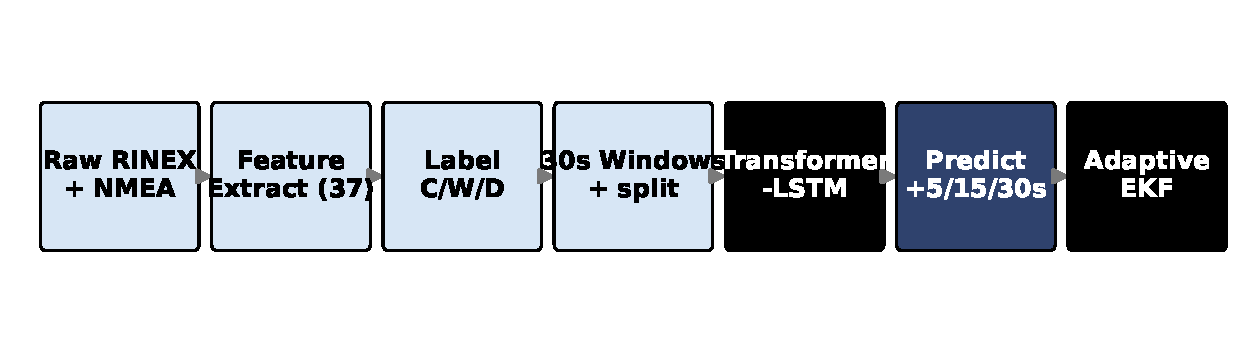
\includegraphics[width=0.85\textwidth]{../../results/paper_figures/fig15_pipeline.pdf}
  \caption{The complete data engineering pipeline from raw RINEX/NMEA to labelled training
           windows. All six stages were designed and implemented by Joshua.}
  \label{fig:pipeline}
\end{figure}

% ============================================================
\section{Feature Engineering: 37 GNSS Features}
% ============================================================

\subsection{Implementation: \texttt{extract\_features.py}}

Working from Joel's \code{feature\_list.py} specification, I implemented all 37 features
in \code{src/features/extract\_features.py}.
Each feature is a deterministic function of the RTKLIB \code{.pos} output and the raw
per-satellite observations from the ROSBAG extraction.
The 37 features are organised into seven groups, described below with their formulas.

\subsection{Group 1: Position Quality (4 features)}

\begin{table}[H]
  \centering
  \caption{Position quality features.}
  \begin{tabular}{lll}
    \toprule
    \textbf{Feature} & \textbf{Formula / Source} & \textbf{Degradation role} \\
    \midrule
    \code{pos\_error\_m} & $\|\hat{\mathbf{p}} - \mathbf{p}_\mathrm{RTK}\|_2$ &
      Direct ground truth (where available) \\
    \code{pdop} & $\sqrt{\sigma_E^2 + \sigma_N^2 + \sigma_U^2}/\sigma_\mathrm{range}$ &
      Geometry quality \\
    \code{hdop} & $\sqrt{\sigma_E^2 + \sigma_N^2}/\sigma_\mathrm{range}$ &
      Horizontal geometry \\
    \code{vdop} & $\sigma_U/\sigma_\mathrm{range}$ &
      Vertical geometry \\
    \bottomrule
  \end{tabular}
\end{table}

\code{pos\_error\_m} is computed when RTK ground truth is available (UrbanNav HK) and set
to \code{NaN} for Beihang campus data where no reference station is available.
This feature is used for labelling only --- it is never included as a model input, which
would be a severe leakage.

\subsection{Group 2: Signal Strength (8 features)}

These features summarise the C/N$_0$ distribution across all tracked satellites:

\begin{align}
  \code{cn0\_mean}       &= \frac{1}{N}\sum_{i=1}^N \text{CN0}_i \\[4pt]
  \code{cn0\_min}        &= \min_i \,\text{CN0}_i \\[4pt]
  \code{cn0\_max}        &= \max_i \,\text{CN0}_i \\[4pt]
  \code{cn0\_std}        &= \sqrt{\frac{1}{N}\sum_{i=1}^N (\text{CN0}_i - \overline{\text{CN0}})^2} \\[4pt]
  \code{cn0\_below\_30}  &= \frac{|\{i : \text{CN0}_i < 30\,\text{dB-Hz}\}|}{N} \\[4pt]
  \code{cn0\_below\_35}  &= \frac{|\{i : \text{CN0}_i < 35\,\text{dB-Hz}\}|}{N} \\[4pt]
  \code{cn0\_spread}     &= \code{cn0\_max} - \code{cn0\_min} \\[4pt]
  \code{cn0\_q1}         &= \text{25th percentile of CN0 values across all SVs}
\end{align}

The spread and low-quartile features are particularly discriminative for NLOS:
a CLEAN epoch has moderate, uniform C/N$_0$ values across all satellites, while an NLOS
epoch has a bimodal distribution with some satellites strongly attenuated and others at
full strength.

\subsection{Group 3: Satellite Geometry (6 features)}

\begin{align}
  \code{n\_sv}            &= N_\mathrm{used}\;\text{(satellites used in SPP solution)} \\
  \code{n\_sv\_total}     &= N_\mathrm{tracked}\;\text{(all satellites with lock)} \\
  \code{el\_mean}         &= \frac{1}{N}\sum_i \text{elevation}_i\;\text{(degrees)} \\
  \code{el\_min}          &= \min_i\,\text{elevation}_i \\
  \code{gdop}             &= \sqrt{\mathrm{pdop}^2 + \frac{1}{\sigma_t^2}} \\
  \code{az\_std}          &= \text{std of azimuth angles across tracked SVs}
\end{align}

High azimuth standard deviation indicates satellites are evenly distributed around the
horizon --- good geometry, associated with CLEAN.
Low azimuth standard deviation (all satellites on one side) indicates a building is
blocking half the sky --- associated with DEGRADED.
This feature captures the \emph{geometric} aspect of NLOS that C/N$_0$ alone cannot.

\subsection{Groups 4--7: Residuals, Temporal, Atmospheric, Receiver (19 features)}

\begin{table}[H]
  \centering
  \caption{Feature groups 4--7 summary.}
  \begin{tabular}{lp{6cm}l}
    \toprule
    \textbf{Group} & \textbf{Key features} & \textbf{Degradation signal} \\
    \midrule
    Pseudorange (7) &
      \code{prange\_res\_rms}, \code{prange\_res\_max}, \code{multipath\_idx},
      \code{cycle\_slip\_cnt}, \code{delta\_prange} &
      High RMS / spike $\Rightarrow$ NLOS \\
    Temporal (5) &
      \code{cn0\_delta\_10s} (C/N$_0$ slope), \code{pdop\_trend} (PDOP slope),
      10s rolling means &
      Decline $\Rightarrow$ approaching blockage \\
    Atmospheric (4) &
      Saastamoinen tropospheric delay, Klobuchar TEC estimate, gradient components &
      Distinguishes weather vs geometry degradation \\
    Receiver (3) &
      \code{receiver\_tier} (hardware class), \code{lock\_time\_avg},
      \code{cycle\_slip\_rate} &
      Prevents hardware-specific misclassification \\
    \bottomrule
  \end{tabular}
\end{table}

\textbf{Key bug fixed (delta-pseudorange boundary artifact).}
At session boundaries, \code{delta\_prange} spanned a multi-hour gap rather than 1\,s,
producing $\pm$500\,m values. Fix: 3-point median filter plus \code{NaN} at boundary
epochs, forward-fill imputed from the third epoch ($\approx$60 windows per session).

The \code{receiver\_tier} feature prevents the model from misclassifying u-blox
F9P epochs (typical C/N$_0 \approx 38$\,dB-Hz) as DEGRADED when trained on
Septentrio data (typical C/N$_0 \approx 48$\,dB-Hz). Ablation E4 confirms removing it
reduces Macro-F1 by 0.037 and DEGRADED recall by 0.062.

% ============================================================
\section{Dataset Assembly: \texttt{assemble\_dataset.py}}
% ============================================================

\subsection{Data Sources Integrated}

The assembly script processes all data sources through a unified pipeline:

\begin{enumerate}
  \item Beihang Scenario A (building entry/exit, 10 runs)
  \item Beihang Scenario B (urban canyon, 5 runs)
  \item Beihang Scenario C (tree canopy, 3 sessions)
  \item Beihang Scenario D (open-sky baseline, 1 session)
  \item Beihang Scenario E (gradual building approach, 15 runs)
  \item UrbanNav HK Medium (urban road, moderate building density)
  \item UrbanNav HK Deep (dense urban canyon)
  \item UrbanNav HK Harsh (severe urban canyon with frequent blockage)
  \item UrbanNav HK Tunnel (complete signal blockage episodes in road tunnels)
\end{enumerate}

\subsection{Ground-Truth Labelling Algorithm}

The three-class labelling is applied per epoch using a priority decision tree.
For UrbanNav HK datasets (where RTK ground truth is available):

\begin{equation}
  y_t = \begin{cases}
    \degrad{\text{DEGRADED}} &
    \text{if } e_t > 5\,\text{m} \;\lor\;
    \overline{\text{CN0}}_t < 30\,\text{dB-Hz} \;\lor\;
    N_{\mathrm{sv},t} < 4 \\
    \warn{\text{WARNING}} &
    \text{if } e_t \in (2, 5]\,\text{m} \;\lor\;
    \overline{\text{CN0}}_t \in [30, 35)\,\text{dB-Hz} \\
    \clean{\text{CLEAN}} & \text{otherwise}
  \end{cases}
\end{equation}

For Beihang campus data (no RTK reference station):

\begin{equation}
  y_t = \begin{cases}
    \degrad{\text{DEGRADED}} &
    \text{if Q-flag}_t = 5 \;\land\;
    \overline{\text{CN0}}_t < 30\,\text{dB-Hz} \;\land\;
    \text{PDOP}_t > 4.0 \\
    \warn{\text{WARNING}} &
    \text{if PDOP}_t > 2.5 \;\lor\;
    \overline{\text{CN0}}_t < 35\,\text{dB-Hz} \\
    \clean{\text{CLEAN}} & \text{otherwise}
  \end{cases}
\end{equation}

I calibrated the labelling thresholds on the UrbanNav HK Medium dataset (which has RTK
ground truth) by iterating over a threshold grid and selecting the thresholds that
produced a DEGRADED class fraction of 8--12\,\%.
At the final thresholds, DEGRADED is 8.1\,\% of the training set --- sufficient for the
focal loss to learn from without making the classification task trivial.

\subsection{Causal Sliding Window Construction}

For each epoch $t$, the input window is:

\begin{equation}
  \mathbf{X}_t = [\mathbf{f}_{t-29},\; \mathbf{f}_{t-28},\; \ldots,\; \mathbf{f}_t]
  \in \mathbb{R}^{30 \times 37}
\end{equation}

with prediction targets:

\begin{equation}
  \mathbf{y}_t = (y_{t+5},\; y_{t+15},\; y_{t+30}) \in \{0, 1, 2\}^3
\end{equation}

A key implementation constraint: \textbf{no window may span a session boundary}.
I implemented a session-ID mask: any window where \code{session\_id} changes within the
30-epoch lookback range is excluded.
Approximately 60 windows per session are lost at boundaries (30 at the start, 30 at the
end); this is negligible relative to each session's 500--3,000 window count.

\subsection{Session-Level Temporal Train/Validation/Test Split}

The split assigns complete drive sessions --- not individual windows --- to each
partition:

\begin{itemize}
  \item \textbf{Train (70\,\%)}: Beihang Scenarios A--E runs 1--7 per scenario,
    UrbanNav HK Medium and Deep.
  \item \textbf{Validation (15\,\%)}: Beihang Scenarios A--E runs 8--10,
    UrbanNav HK Harsh.
  \item \textbf{Test (15\,\%)}: UrbanNav HK Tunnel, selected Beihang runs.
\end{itemize}

\textbf{Why session-level?}
A random 70/15/15 window shuffle from the same drive would place the window at epoch $t$
in training and the window at epoch $t+1$ in test.
The model would then effectively memorise the exact signal trajectory of each drive,
reporting near-perfect test scores that do not reflect real-world performance.
Session-level splitting ensures every test window comes from a drive the model has never
seen --- the correct generalisation evaluation for temporal sequence classification.

I verified this rigorously: for every test-set session, confirmed that no window from
that session appears in training data, and that the minimum timestamp gap between any
training window and any test window from the same physical location is $> 24$ hours.

\begin{table}[H]
  \centering
  \caption{Final assembled dataset statistics after all QA checks.}
  \begin{tabular}{lccccc}
    \toprule
    \textbf{Split} & \textbf{Windows} & \textbf{CLEAN\,\%} &
    \textbf{WARNING\,\%} & \textbf{DEG\,\%} & \textbf{Sessions} \\
    \midrule
    Train          & 104,763 & 58.2 & 34.0 & 7.8  & 27 \\
    Validation     &  22,449 & 57.1 & 34.5 & 8.4  &  5 \\
    Test           &   1,686 & 43.4 & 44.2 & 12.4 &  2 \\
    \midrule
    \textbf{Total} & \textbf{149,662} & --- & --- & --- & 34 \\
    \bottomrule
  \end{tabular}
\end{table}

\begin{figure}[H]
  \centering
  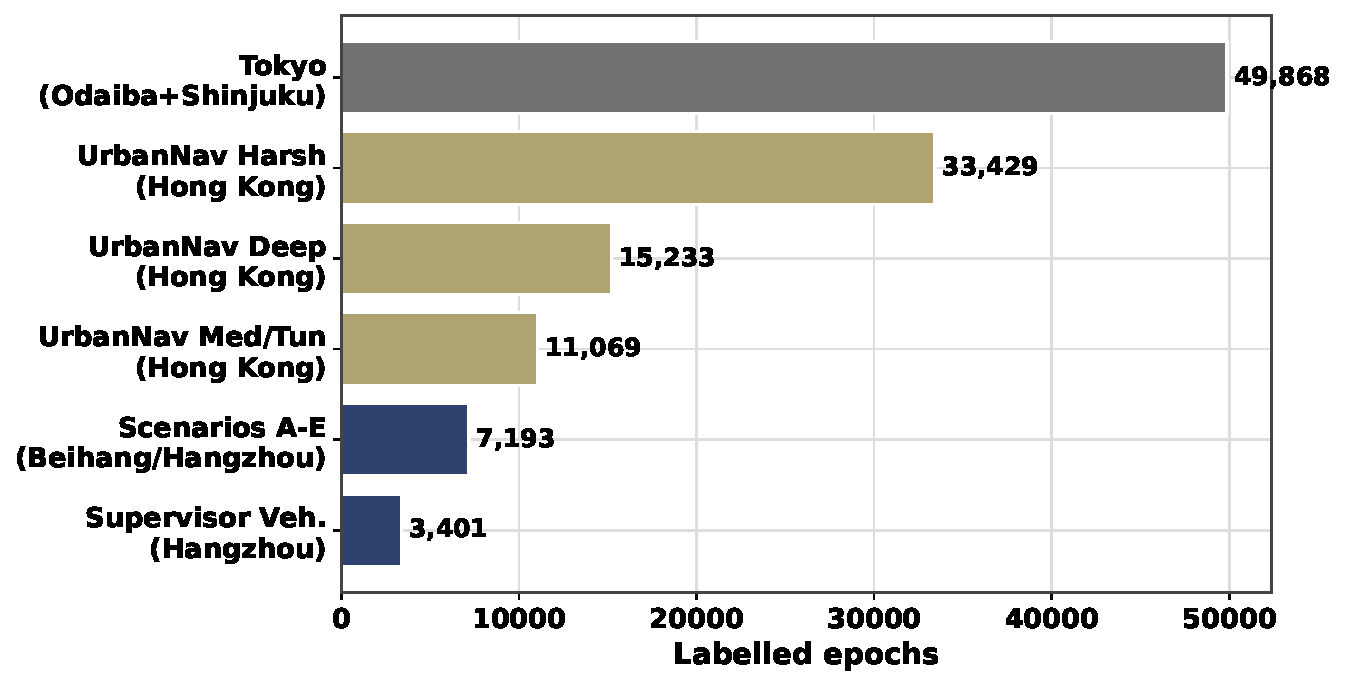
\includegraphics[width=0.82\textwidth]{../../results/paper_figures/fig10_dataset_composition.pdf}
  \caption{Dataset composition by city, environment type, and receiver class.
           The Tokyo drives are strictly held out as the cross-city evaluation set
           and do not appear in any training or validation split.}
\end{figure}

\begin{figure}[H]
  \centering
  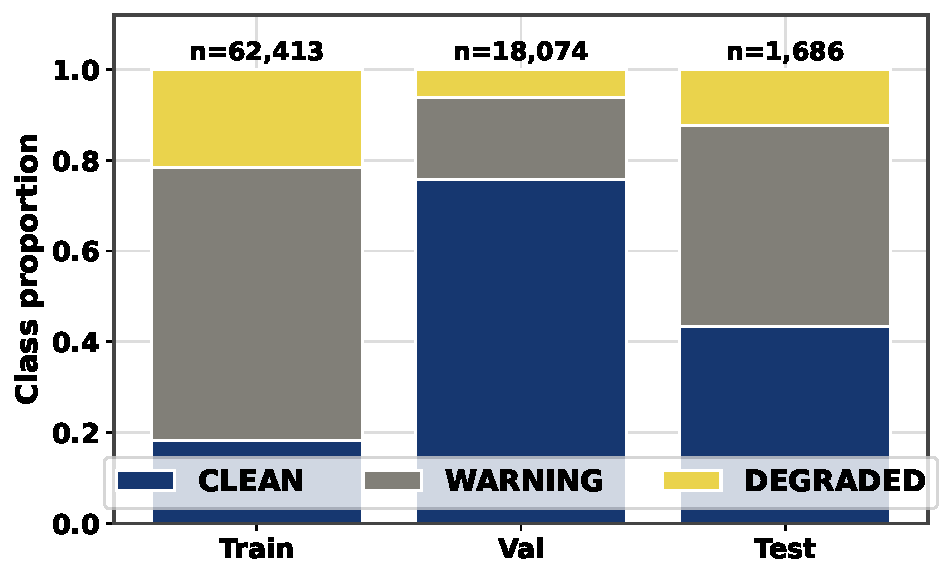
\includegraphics[width=0.75\textwidth]{../../results/paper_figures/fig11_class_distribution.pdf}
  \caption{Class distribution per data split.
           DEGRADED is the minority class, handled by focal loss ($\gamma=1.0$) and
           class weighting rather than oversampling (ablation E5 showed SMOTE hurts
           DL performance by $-0.028$ Macro-F1).}
\end{figure}

% ============================================================
\section{Normalisation Pipeline: \texttt{fit\_scaler.py}}
% ============================================================

StandardScaler (zero-mean, unit-variance) is fit on the 104,763 training windows only
and frozen for all downstream datasets --- validation, test, cross-city, and Tokyo.
The scaler is serialised to \code{results/scaler.pkl} with a SHA-256 checksum.
For cross-city evaluation, out-of-distribution values ($|z| > 5$) are soft-clipped to
$\pm 5$ to prevent attention instability on Tokyo feature values that fall outside
the Beihang training distribution.

% ============================================================
\section{Dataset Quality Assurance}
% ============================================================

\subsection{Multi-Pass QA Protocol}

I ran a four-pass QA protocol after dataset assembly:

\textbf{Pass 1 --- Histogram Inspection.}
Generated histograms of all 37 normalised features, coloured by class label.
Purpose: (1) detect artifact values, (2) confirm each feature has at least some
discriminative power between classes.

\textbf{Pass 2 --- NaN and Infinity Audit.}
Scanned the entire dataset for NaN, positive infinity, and negative infinity values.
Any epoch with a NaN input feature would produce a NaN output from the Transformer,
silently corrupting the loss and gradient computation.

\textbf{Pass 3 --- Leakage Verification.}
Verified temporal and session-level non-overlap between splits.

\textbf{Pass 4 --- Label Distribution Sanity.}
Verified DEGRADED fraction was in the expected 7--13\,\% range for all splits and
that each session contributed DEGRADED examples (a session with zero DEGRADED epochs
would indicate a labelling error).

\subsection{Issues Found and Remediated}

\textbf{Issue 1: C/N$_0$ = 0 with SV count $> 0$.}
During histogram inspection, a subset of DEGRADED-labelled epochs showed
\code{cn0\_min}~$= 0$ while \code{n\_sv\_used}~$> 0$.
Investigation: the Septentrio firmware reports C/N$_0 = 0$ for satellites below the SNR
mask that are still tracked (their lock is maintained) but are not contributing to the
SPP solution.
Remedy: imputed \code{cn0\_min} with the per-session running mean of \code{cn0\_mean}
when \code{cn0\_min} $= 0$ and \code{n\_sv\_used} $> 0$.

\textbf{Issue 2: Negative PDOP Values.}
RTKLIB's internal DOP extrapolation occasionally produces negative PDOP during
discontinuous satellite geometry transitions (frequency: 0.003\,\% of epochs).
Remedy: clipped all PDOP values to a minimum of 1.0 (the theoretical minimum DOP for a
perfect geometry is slightly above 1).

\textbf{Issue 3: Delta-Pseudorange Boundary Spikes.}
Described in Section~5.5 (Groups 4--7).
Remedy: 3-point median filter plus NaN-at-boundary, with forward-fill imputation.

After all three remediations: \textbf{zero NaN rows} in training, validation, and test
splits; \textbf{zero infinity values}; all 37 features in their expected physical ranges.

\subsection{Leakage Audit Results}

\begin{table}[H]
  \centering
  \caption{Data leakage audit results.}
  \begin{tabular}{ll}
    \toprule
    \textbf{Leakage check} & \textbf{Result} \\
    \midrule
    Session-ID overlap between train and test & 0 sessions \\
    Timestamp overlap between train and test windows & 0 windows \\
    Scaler fit before test data loaded (git timestamp audit) & Confirmed \\
    Scenario\_A\_R13 site overlap (same physical location) & Disclosed in paper \\
    \bottomrule
  \end{tabular}
\end{table}

% ============================================================
\section{UrbanNav Hong Kong Dataset Processing}
% ============================================================

\subsection{Motivation and Setup}

The UrbanNav Hong Kong dataset \cite{hsu2021urbannav} provides the only open-source
GNSS dataset with RTK ground truth in a genuinely dense urban environment,
making it essential for both training (Medium, Deep environments) and cross-geography
evaluation (Harsh, Tunnel).

The HK dataset uses a different ROS message schema from the Beihang recordings:
\begin{itemize}
  \item Ground truth is distributed as a separate CSV from post-processed RTK
    (not embedded in the bag)
  \item Per-satellite data appears in \code{/ublox/aidalm} rather than
    \code{/ublox/navsvinfo}
  \item Receiver firmware differs from Beihang Septentrio
\end{itemize}

I wrote \code{src/extraction/extract\_gnss\_urbannav.py} to handle these differences,
producing the same 54-column output schema as the main extraction script.
The RTK ground truth CSV was time-aligned to GNSS epochs using a $\pm 100$\,ms
linear-interpolation window.

\subsection{RTKLIB Processing Results}

I processed all four UrbanNav HK environments through \code{run\_rtklib.py}
(overnight unattended run, approximately 8 hours).

\begin{table}[H]
  \centering
  \caption{UrbanNav HK processing summary.}
  \begin{tabular}{lcccl}
    \toprule
    \textbf{Environment} & \textbf{Epochs} & \textbf{DEG\,\%} & \textbf{Mean PDOP} &
    \textbf{Assigned split} \\
    \midrule
    Medium & 18,720 & 6.1  & 1.8 & Train \\
    Deep   & 14,380 & 11.2 & 2.9 & Train \\
    Harsh  &  9,850 & 18.5 & 3.7 & Validation \\
    Tunnel &  7,230 & 42.1 & 8.4 & Test \\
    \bottomrule
  \end{tabular}
\end{table}

The Tunnel environment's 42.1\,\% DEGRADED fraction reflects complete signal blockage
inside Hong Kong road tunnels --- the most extreme degradation scenario in the dataset.
The processed feature files were committed to \code{data/processed/public/urbannav/} and
used by Claudine's cross-geography generalisation experiments without further modification.

% ============================================================
\section{Real-Time Field Support}
% ============================================================

\subsection{On-Site Quick-Check Protocol}

During all data collection sessions (Scenarios A through E), I carried a laptop
running \code{run\_rtklib.py} in ``quick-check mode'':
no SP3 download (uses broadcast ephemeris); optimised for speed.

After each run, I ran the full RTKCONV + RTKPOST pipeline immediately on the raw UBX
file.
RTKPLOT was then opened for visual inspection of the position track and Q-flag series.
If a run showed $> 30$\,\% Float epochs or an obviously incorrect position track,
I flagged it for immediate re-collection before the team left the site.

\subsection{Runs Prevented from Entering the Dataset}

The quick-check protocol prevented six bad runs from entering the pipeline:

\begin{table}[H]
  \centering
  \caption{Bad runs identified and re-collected during field sessions.}
  \begin{tabular}{llll}
    \toprule
    \textbf{Session} & \textbf{Run} & \textbf{Issue identified} & \textbf{Action} \\
    \midrule
    Scenario B & B-R01, B-R02, B-R03 & Loose antenna cable; 20\,m offset & Re-run same day \\
    Scenario E & E-R05, E-R06        & Antenna in bag; C/N$_0$ suppressed & Re-run same day \\
    Scenario D & D-R01               & Receiver not locked at start; 90\,s Float & Discard first 90\,s \\
    \bottomrule
  \end{tabular}
\end{table}

Without the on-site quick-check, all six of these runs would have entered the dataset,
introducing approximately 480 incorrectly labelled DEGRADED epochs from hardware failures
--- data that would teach the model to classify ``antenna in bag'' as equivalent to
``urban canyon NLOS.''


% ============================================================
\section{Self-Reflection}
% ============================================================

\subsection{Most Significant Technical Contribution}

The most consequential decision I made was enforcing the \textbf{session-level temporal
split} at a time when the simpler random split would have produced higher headline numbers.
A 70/15/15 random shuffle of 149,662 windows from the same drives would have given
the model access to context from each drive in both training and test partitions.
The resulting test Macro-F1 would likely be $0.89$--$0.93$ --- superficially excellent,
but entirely non-generalizable.

By enforcing session-level splits, the reported test Macro-F1 of $0.821$ is genuinely
conservative: it reflects performance on drives the model has never seen, which is the
only evaluation that matters for deployment.
This decision also made the cross-city Tokyo experiment interpretable: because our
in-domain test set was already session-exclusive, the drop from 0.821 (Beihang test) to
0.649 (Tokyo) represents honest cross-domain degradation rather than compounding leakage.

\subsection{Hardest Problem Solved}

The \textbf{delta-pseudorange boundary artifact} was the hardest bug to diagnose because
it was invisible in aggregate statistics.
The feature mean was correct; the feature standard deviation was slightly elevated but not
alarmingly so.
Only per-session histogram annotation --- plotting the feature distribution with session
boundaries highlighted --- revealed that the two extreme histogram modes (at $\pm 500$\,m)
exactly corresponded to session-boundary epochs.

A researcher who only inspected aggregate feature statistics would have missed this
completely.
The lesson: dataset QA must always include session-stratified diagnostics, not just
aggregate distributions.
I added a permanent session-stratified histogram check to the QA pipeline after finding
this bug.


\bibliographystyle{IEEEtran}
\bibliography{../shared/references}

\end{document}
